\documentclass[a4paper]{scrreprt}

\usepackage[german]{babel}
\usepackage[utf8]{inputenc}
\usepackage[T1]{fontenc}
\usepackage{ae}
\usepackage[bookmarks,bookmarksnumbered]{hyperref}
\usepackage{graphicx}
\usepackage{parskip}
\usepackage[toc]{glossaries}
\usepackage{tocbasic}
\usepackage{booktabs}
\usepackage{float}
\usepackage{wrapfig}
\graphicspath{ {images/} }
\setcounter{secnumdepth}{5}
\makeglossaries
\renewcommand{\arraystretch}{1.5}
\setlength{\tabcolsep}{12pt}

\newglossaryentry{android}
{
	name=Android-App, 
	description={Anwendungssoftware für Mobilgeräte mit Android als Betriebssystem}
}   

\begin{document}
    \begin{flushright}
        
\includegraphics[scale = 0.2]{kit-logo.png}\\[0.5cm]
    \end{flushright}
    \vspace*{2cm}

    \begin{center} 
    		\large Praxis der Softwareentwicklung
        \vspace*{1.5cm}

        \textbf{\huge Fridget}
        \vspace*{1cm}

        \textbf{\Large Pflichtenheft}
        \vspace*{2cm}

        Yunjia Chen, Jasmin Jat, Min Hye Park, Alina Shah, Lisa Wang
        \vspace*{1cm}

        27. März 2018
        \vspace*{2.5cm}

        Betreuung: Erik Burger, Sandro Koch\\[0.5cm]
        IPD\\[0.5cm]

        Karlsruher Institut für Technologie
    \end{center}
    \thispagestyle{empty}

    \tableofcontents

    \chapter{Zielbestimmung}
    
    	\section{Einleitung}
    	Im Rahmen des Softwareprojekts PSE entwickelte unser Team die Applikation Fridget. Der Name setzt sich aus den englischen Begriffen für Kühlschrank ``fridge” und Apparat ``gadget” zusammen. Die App ermöglicht es Wohn- und Lebensgemeinschaften, eine Online-Pinnwand zu erstellen und diese mit zahlreichen Notizzetteln zu füllen. Anstelle einer langweiligen Kork-Pinnwand-Ansicht bietet sie, wie der Name schon andeutet, eine moderne Kühlschrank-Ansicht im Retro-Design.\\
    	Unser Ziel ist es, für Studenten das WG-Leben einfacher zu gestalten und ihnen die Möglichkeit zu geben, alle wichtigen WG-Informationen an einem Ort festhalten zu können.
    	
    	\newpage
    
        \section{Musskriterien - KM}
        \begin{table}[h!]
        	\centering
        	\label{my-label}
        	\begin{tabular}{p{2cm}p{12cm}}
        		
        		\multicolumn{2}{c}{\textbf{1 - Erstellen einer WG-Pinnwand}} \\ \hline
        		\centering{[}KM1010{]} & Eine Person muss sich in der App mit einem Google Account registrieren.\\
        		\centering{[}KM1020{]}& Ein Benutzer kann sich mit einem Zugangscode bei einer bestehenden WG-Pinnwand anmelden oder eine neue WG-Pinnwand erstellen.                                 \\
        		\centering{[}KM1030{]}& Beim Erstellen einer neuen WG-Pinnwand gibt der Benutzer der neuen WG-Pinnwand einen Namen.\\ 
        		\centering{[}KM1040{]}& Die Pinnwand ist unterteilt in \textit{Frozen Notes} und \textit{Cool Notes}.\\ 
        		\centering{[}KM1050{]}& Die \textit{Frozen Notes} sind feste, nicht löschbare, bearbeitbare Notizen und werden beim Erstellen der WG generiert.\\ 
        		\centering{[}KM1060{]}& Die \textit{Cool Notes} sind löschbare, nicht bearbeitbare Notizen und werden vom Benutzer erstellt.\\ 
        		\hline
        	\end{tabular}
        \end{table}
    
    	\vspace{5mm}
    	
    	\begin{table}[h!]
    		\centering
    		\label{my-label}
    		\begin{tabular}{p{2cm}p{12cm}}
    			
    			\multicolumn{2}{c}{\textbf{2 - Interaktion mit der Pinnwand}} \\ \hline
    			\centering{[}KM2010{]} & Der Benutzer kann eine \textit{Cool Note} mit einer Überschrift und Textinhalt erstellen und löschen.\\
    			\centering{[}KM2020{]}& Der Benutzer kann die \textit{Frozen Notes} bearbeiten.                                 \\
    			\centering{[}KM2030{]}& Dem Benutzer wird eine Magnetfarbe zugeteilt.\\ 
    			
    			\hline
    		\end{tabular}
    	\end{table}
    
    	\vspace{5mm}
    	
    	\begin{table}[h!]
    		\centering
    		\label{my-label}
    		\begin{tabular}{p{2cm}p{12cm}}
    			
    			\multicolumn{2}{c}{\textbf{3 - Synchronisierung mit dem Server}} \\ \hline
    			\centering{[}KM3010{]} & Der Benutzer kann die App manuell aktualisieren.\\
    			
    			\hline
    		\end{tabular}
    	\end{table}
    
    	\vspace{5mm}
    	
    	\begin{table}[h!]
    		\centering
    		\label{my-label}
    		\begin{tabular}{p{2cm}p{12cm}}
    			
    			\multicolumn{2}{c}{\textbf{4 - App-Menü}} \\ \hline
    			\centering{[}KM4010{]} & Der Benutzer kann eine Liste der Mitglieder und ihre entsprechende Magnetfarbe einsehen.\\
    			\centering{[}KM4020{]}& Der Benutzer kann eine WG verlassen.                               \\
    			\centering{[}KM4030{]}& Die App-Sprache ist Englisch.\\ 
    			
    			\hline
    		\end{tabular}
    	\end{table}
    
    	\vspace{5mm}
    	
    	\begin{table}[h!]
    		\centering
    		\label{my-label}
    		\begin{tabular}{p{2cm}p{12cm}}
    			
    			\multicolumn{2}{c}{\textbf{5 - Lesebestätigung}} \\ \hline
    			\centering{[}KM5010{]} & Der Ersteller sieht, wer seine \textit{Cool Notes} gelesen hat.\\
    			\centering{[}KM5020{]}& Der Benutzer kann markieren, welche \textit{Cool Notes} er gelesen hat.                               \\ 
    			
    			\hline
    		\end{tabular}
    	\end{table}
    
    	\vspace{5mm}
    	
    	\begin{table}[h!]
    		\centering
    		\label{my-label}
    		\begin{tabular}{p{2cm}p{12cm}}
    			
    			\multicolumn{2}{c}{\textbf{6 - Push-Benachrichtigung}} \\ \hline
    			\centering{[}KM5010{]} & Alle Mitglieder bekommen für eine neue \textit{Cool Note} eine Push-Benachrichtigung.\\
    			\centering{[}KM5020{]}& Über die Push-Benachrichtigung gelangt der Benutzer direkt zur neuen \textit{Cool Note}.                               \\
    			
    			\hline
    		\end{tabular}
    	\end{table}
    	
    	\vspace{1cm}    	
    	
    	\clearpage

        \section{Wunschkriterien - KW}
		\begin{table}[h!]
			\centering
			\label{my-label}
			\begin{tabular}{p{2cm}p{12cm}}
				
				\multicolumn{2}{c}{\textbf{1 - Taggen}} \\ \hline
				\centering{[}KW1010{]} & Benutzer können nur in ihrer \textit{Cool Note} einen oder mehrere Mitglieder taggen.\\
				\centering{[}KW1020{]}& Nur die getaggten Mitglieder bekommen eine Push-Benachrichtigung.                               \\
				\hline
			\end{tabular}
		\end{table}
		
		\vspace{5mm}
		
		\begin{table}[h!]
			\centering
			\label{my-label}
			\begin{tabular}{p{2cm}p{12cm}}
				
				\multicolumn{2}{c}{\textbf{2 - Interaktion mit der Pinnwand}} \\ \hline
				\centering{[}KW2010{]} & Beim Erstellen der \textit{Cool Notes} kann deren Wichtigkeit durch das Auswählen der Zettelfarbe festgelegt und angezeigt werden.\\
				\centering{[}KW2020{]}& Der Benutzer kann eine \textit{Cool Note} mit einer Beschreibung und Bildinhalt erstellen und löschen.                              \\
				\centering{[}KW2030{]}& Benutzer können unter \textit{Cool Notes} Kommentare schreiben.\\ 
				\centering{[}KW2040{]}& Der Benutzer kann eine \textit{Cool Note} archivieren.\\ 
				\hline
			\end{tabular}
		\end{table}
		
		\vspace{5mm}
		
		\begin{table}[h!]
			\centering
			\label{my-label}
			\begin{tabular}{p{2cm}p{12cm}}
				
				\multicolumn{2}{c}{\textbf{3 - App-Menü}} \\ \hline
				\centering{[}KW3010{]} & Die App kann auf mehrere Sprachen umgestellt werden.\\
				\centering{[}KW3020{]} & Der Benutzer kann archivierte \textit{Cool Notes} aufrufen.\\
				\hline
			\end{tabular}
		\end{table}
		
		\vspace{5mm}
		
		\begin{table}[h!]
			\centering
			\label{my-label}
			\begin{tabular}{p{2cm}p{12cm}}
				
				\multicolumn{2}{c}{\textbf{4 - Hilfe-Button}} \\ \hline
				\centering{[}KM4010{]} & Beim Drücken des Buttons erscheint ein Tutorial-Overlay.\\
				
				
				\hline
			\end{tabular}
		\end{table}
	
		\vspace{1cm}
		\clearpage
		
        \section{Abgrenzungskriterien - KA}
        
        \begin{table}[h!]
        	\centering
        	\label{my-label}
        	\begin{tabular}{p{2cm}p{12cm}}
        		
        		\multicolumn{2}{c}{\textbf{1.3}} \\ \hline
        		\centering{[}KA1010{]} & Die App kann nicht im Querformat benutzt werden.\\
        		\centering{[}KA1020{]}& Keine Browserapp ist geplant.                                 \\
        		\centering{[}KA1030{]}& Man kann nur Mitglieder einer WG sein.\\ 
        		\centering{[}KA1040{]}& Eine WG kann nicht mehr als 15 Mitglieder haben..\\ 
        		\centering{[}KA1050{]}& \textit{Cool Notes} können nicht bearbeitet werden.\\ 
        		\centering{[}KA1060{]}& Es können nicht mehr als neun \textit{Cool Notes} pro Pinnwand erstellt werden.\\ 
        		\centering{[}KA1070{]}& Jedes Mitglied kann nur ein Kommentar pro Note schreiben.\\ 
        		\hline
        	\end{tabular}
        \end{table}

    \chapter{Produkteinsatz}
    
        \documentclass[a4paper]{scrreprt}

\usepackage[german]{babel}
\usepackage[utf8]{inputenc}
\usepackage[T1]{fontenc}
\usepackage{ae}

\begin{document}
    \chapter{Produkteinsatz}
        \section{Anwendungsbereiche}
        Die App ist in einem gemeinsamen Haushalt einsetzbar, um wichtige interne Informationen unmittelbar unter allen Mitbewohnern auszutauschen.
        
        \section{Produktumgebung}
        \begin{tabular}{|l|l|p{.6\textwidth}|}
        \hline
        \multicolumn{3}{|l|} {Server} \\
        \hline
        Container & Docker & Die Serverseitigen Softwares werden in einem Docker Container verpackt. \\ \hline
        Webserver & Tomcat & Zum Übertragen von Daten an Client durch HTTP-Anfrage. \\ \hline
        Datenbank & MySQL & Zum Speichern und Verwalten von Daten. \\
        \hline \hline
        \multicolumn{3}{|l|}{Client} \\
        \hline
        Mobile Betriebssystem & \multicolumn{2}{|l|}{Android 5.1 Lollipop} \\ \hline
        \end{tabular}
        
        \section{Betriebsbedingungen}
        Zur Anmeldung wird ein bereits vorhandenes Google-Konto benötigt. \\
        Zum App-Betrieb wird eine aktive Internetverbindung zum Server benötigt. Ohne eine bestehende Verbindung können weder die Notizen synchronisiert noch Benachrichtigungen erhalten werden.

        \section{Zielgruppen}
        Haupt-Zielgruppe der App sind die Personen, die in einer Wohngemeinschaft oder Haushaltsgemeinschaft leben. Ebenfalls kann sie von kleinen Gruppen genutzt werden, die nicht zusammen wohnen sich jedoch trotzdem verbinden möchten.

\end{document}

    \chapter{Produktfunktionen}
    		\section{Grundfunktionen - FG}
    		
    		\begin{table}[h!]
    			\centering
    			\label{my-label}
    			\begin{tabular}{p{2cm}p{12cm}}
    				
    				\multicolumn{2}{c}{\textbf{1 - Erstellen einer WG-Pinnwand}} \\ \hline
    				\centering{[}FG1010{]} & Registrierung durch ein Google-Account {[}KM1010{]}\\
    				\centering{[}FG1020{]}& Erstellen einer neuen WG Pinnwand mit Namen {[}KM1020{]} {[}KM1030{]}                                \\
    				\centering{[}FG1030{]}& Generierung eines zufälligen Zugangscode aus Nummern und Buchstaben {[}KM1020{]} {[}KM1030{]}\\ 
    				\centering{[}FG1040{]}& Anmelden mit Zugangscode {[}KM1020{]}\\ 
    				\centering{[}FG1050{]}& Generieren und Anzeigen von drei \textit{Frozen Notes} {[}KM1050{]}\\ 
    				\hline
    			\end{tabular}
    		\end{table}
    		
    		\vspace{5mm}
    		
    		\begin{table}[h!]
    			\centering
    			\label{my-label}
    			\begin{tabular}{p{2cm}p{12cm}}
    				
    				\multicolumn{2}{c}{\textbf{2 - Interaktion mit der Pinnwand}} \\ \hline
    				\centering{[}FG2010{]} & Erstellen einer \textit{Cool Note} mit obligatorischer Überschrift und optionalem Textinhalt {[}KM2010{]}\\
    				\centering{[}FG2020{]}& Unterstreichen, Kursiv-Schreiben oder Fett-Drucken von Textinhalten in Cool und \textit{Frozen Notes} {[}KM2010{]}                              \\
    				\centering{[}FG2030{]}& Zufällige Positionierung der \textit{Cool Note} mit Überschrift und entsprechender Magnetfarbe auf der Pinnwand {[}KM2010{]} {[}KM2030{]}\\ 
    				\centering{[}FG2040{]}& Öffnen einer Frozen oder \textit{Cool Note} durch Antippen {[}KM2010{]} {[}KM2020{]}\\ 
    				\centering{[}FG2050{]}& Löschen einer \textit{Cool Note} mit Textinhalt und Überschrift {[}KM2010{]}\\ 
    				\centering{[}FG2060{]}& Bearbeitung der \textit{Frozen Notes} {[}KM2020{]}\\ 
    				\centering{[}FG2070{]}& Zuordnung unterschiedlicher Magnetfarben pro Mitglied {[}KM2030{]}\\ 
    				\centering{[}FG2080{]}& Manuelle Aktualisierung der Pinnwand durch Hinunterswipen {[}KM3010{]}\\ 
    				\hline
    			\end{tabular}
    		\end{table}
    		
    		\vspace{5mm}
    		
    		\begin{table}[h!]
    			\centering
    			\label{my-label}
    			\begin{tabular}{p{2cm}p{12cm}}
    				
    				\multicolumn{2}{c}{\textbf{3 - App-Menü}} \\ \hline
    				\centering{[}FG3010{]} & Verlassen der WG und Löschen aller vorhandenen \textit{Cool Notes} der Verlassenden {[}KM4020{]}\\
    				\centering{[}FG3020{]} & Anzeigen und Scrollen von Mitgliederliste {[}KM4010{]}\\
    				\centering{[}FG3030{]} & Automatisches Aktualisieren der Mitgliederliste {[}KM4010{]}\\
    				\hline
    			\end{tabular}
    		\end{table}
    		
    		\vspace{5mm}
    		
    		\begin{table}[h!]
    			\centering
    			\label{my-label}
    			\begin{tabular}{p{2cm}p{12cm}}
    				
    				\multicolumn{2}{c}{\textbf{4 - Lesebestätigung}} \\ \hline
    				\centering{[}FG4010{]} & Anzeigen der Leser einer \textit{Cool Note} {[}KM5010{]}\\
    				\centering{[}FG4020{]}& Darstellen einer ``I have seen this”-Checkbox {[}KM5020{]}                              \\
    				\centering{[}FG4030{]}& Speichern der Checkbox-Markierung {[}KM5020{]}\\ 
    				
    				\hline
    			\end{tabular}
    		\end{table}
    		
    		\vspace{5mm}
    		
    		\begin{table}[h!]
    			\centering
    			\label{my-label}
    			\begin{tabular}{p{2cm}p{12cm}}
    				
    				\multicolumn{2}{c}{\textbf{5 - Push-Benarichtigung}}\\ \hline
    				\centering{[}FG5010{]} & Generieren und Abschicken der Push-Benachrichtigung {[}KM6010{]}\\
    				\centering{[}FG5020{]}&Öffnen der Großansicht der neuen Notiz direkt durch die Push-Benachrichtigung {[}KM6020{]}           \\ 
    				
    				\hline
    			\end{tabular}
    		\end{table}
    		
    		\vspace{1cm}
    		\clearpage
    		
    		\section{Optionale Funktionen - FO}
    		
    		\begin{table}[h!]
    			\centering
    			\label{my-label}
    			\begin{tabular}{p{2cm}p{12cm}}
    				
    				\multicolumn{2}{c}{\textbf{1 - Taggen}} \\ \hline
    				\centering{[}FO1010{]} & Taggen von anderen Mitgliedern mit ``@”-Zeichen im Content-Feld {[}KW1010{]}\\
    				\centering{[}FO1020{]}& Anzeigen von Namensvorschlägen bei der Eingabe von ``@” {[}KW1010{]} \\
    				\hline
    			\end{tabular}
    		\end{table}
    		
    		\vspace{5mm}
    		
    		\begin{table}[h!]
    			\centering
    			\label{my-label}
    			\begin{tabular}{p{2cm}p{12cm}}
    				
    				\multicolumn{2}{c}{\textbf{2 - Interaktion mit der Pinnwand}} \\ \hline
    				\centering{[}FO2010{]} & Festlegen der Zettelfarben {[}KW2010{]}\\
    				\centering{[}FO2020{]}& Erstellen einer \textit{Cool Note} mit Bildinhalt und Beschreibung {[}KW2020{]}     \\
    				\centering{[}FO2030{]}& Löschen einer \textit{Cool Note} mit Bildinhalt und Beschreibung {[}KW2020{]}\\ 
    				\centering{[}FO2040{]}& Kommentieren der \textit{Cool Notes} {[}KW2030{]}\\ 
    				\centering{[}FO2050{]}& Archivieren einer \textit{Cool Note} {[}KW2040{]}\\ 
    				\centering{[}FO2060{]}& Scrollen von den Kommentaren in den \textit{Cool Notes} {[}KW2030{]}\\ 
    				\hline
    			\end{tabular}
    		\end{table}
    		
    		\vspace{5mm}
    		
    		\begin{table}[h!]
    			\centering
    			\label{my-label}
    			\begin{tabular}{p{2cm}p{12cm}}
    				
    				\multicolumn{2}{c}{\textbf{3 - App Einstellungen / App-Menü}} \\ \hline
    				\centering{[}FO3010{]} & Umstellen der App-Sprache {[}KW3010{]}\\
    				\centering{[}FO3020{]} & Aufrufen und Scrollen von dem Cool-Note-Archiv {[}KW3020{]}\\
    				\hline
    			\end{tabular}
    		\end{table}
    		
    		\vspace{5mm}
    		
    		\begin{table}[h!]
    			\centering
    			\label{my-label}
    			\begin{tabular}{p{2cm}p{12cm}}
    				
    				\multicolumn{2}{c}{\textbf{4 - Hilfe-Button / ``Tutorial"}} \\ \hline
    				\centering{[}FO4010{]} & Ansehen des Tutorial-Overlays {[}KW4010{]}\\    				
    				\hline
    			\end{tabular}
    		\end{table}
    		
    		\vspace{1cm}
    		
    		\newpage
    		
    		\section{Produktleistungen - FL}
    		Durch die variierende Geschwindigkeit der Internet- und Serververbindungen werden uns technische Grenzen aufgezeigt, die wir nicht kontrollieren können. Deswegen können wir keinerlei Angaben zu zeitlichen Produktleistungen machen, welche diese Funktionen benötigen. 
    		\\
    		
    		\begin{table}[h!]
    			\centering
    			\label{my-label}
    			\begin{tabular}{p{2cm}p{12cm}}
    				
    				\multicolumn{2}{c}{\textbf{1 - Erstellen einer WG-Pinnwand}} \\ \hline
    				\centering{[}FL1010{]} & Nach dem Öffnen der App darf es nicht länger als 15 Sekunden dauern, bis das (Registrierungsfenster) Anmeldefenster angezeigt wird \\
    				\hline
    			\end{tabular}
    		\end{table}
    		
    		\vspace{5mm}
    		
    		\begin{table}[h!]
    			\centering
    			\label{my-label}
    			\begin{tabular}{p{2cm}p{12cm}}
    				
    				\multicolumn{2}{c}{\textbf{2 - Interaktion mit der Pinnwand}} \\ \hline
    				\centering{[}FL2010{]} & Pro Pinnwand können drei \textit{Frozen Notes} und neun \textit{Cool Notes} dargestellt werden.\\
    				\centering{[}FL2020{]}& Es müssen maximal 15 Teilnehmer verwaltet werden können.                             \\ 
    				\hline
    			\end{tabular}
    		\end{table}
    		
    		\vspace{5mm}
    		
    		\begin{table}[h!]
    			\centering
    			\label{my-label}
    			\begin{tabular}{p{2cm}p{12cm}}
    				
    				\multicolumn{2}{c}{\textbf{3 - App Einstellungen / App-Menü}} \\ \hline
    				\centering{[}FL3010{]} & Als Standard-Sprache für die grafische Oberfläche ist Englisch voreingestellt.\\
    				\hline
    			\end{tabular}
    		\end{table}
    		
    		\vspace{5mm}
    		
    		\begin{table}[h!]
    			\centering
    			\label{my-label}
    			\begin{tabular}{p{2cm}p{12cm}}
    				
    				\multicolumn{2}{c}{\textbf{4 - Zeichenbegrenzung}} \\ \hline
    				\centering{[}FL4010{]} & Die Überschrift ist durch 20 Zeichen begrenzt.\\
    				\centering{[}FL4020{]}& Der Textinhalt ist durch 300 Zeichen begrenzt.                              \\
    				\hline
    			\end{tabular}
    		\end{table}
    		
    		
    		\newpage
    		
    		\section{Qualitäts-Zielbestimmung}
    		
    	\begin{table}[h!]
    		\centering
    		\begin{tabular}{llll}
    			\multicolumn{1}{l}{\textit{Produktqualität}}& \multicolumn{1}{c}{\textit{Sehr hoch}} & \multicolumn{1}{c}{\textit{Hoch}} & \multicolumn{1}{c}{\textit{Normal}}  \\
    			\multicolumn{4}{c}{- Funktionalität -} \\
    			RICHTIGKEIT                                  &                                        &    \hspace{6mm}               X               &                                      \\
    			INTEROPERABILITÄT                            &                                        &                                   &    \hspace{6mm}                     X               \\
    			ORDNUNGSMÄSSIGKEIT                           &                                        &                                   &    \hspace{6mm}                     X               \\
    			SICHERHEIT                                   &                                        &                                   &    \hspace{6mm}                     X               \\
    			\multicolumn{4}{c}{- Zuverlässigkeit -}\\
    			REIFE                                        &                                        &                                   &     \hspace{6mm}                    X               \\
    			FEHLERTOLERANZ                               &                                        &  \hspace{6mm}                    X               &                                      \\
    			WIEDERHERSTELLBARKEIT                        &                                        &   \hspace{6mm}                   X               &                                      \\
    			STABILITÄT                                   &                                        &  \hspace{6mm}                    X               &                                      \\
    			\multicolumn{4}{c}{- Benutzbarkeit -}\\
    			VERSTÄNDLICHKEIT                             &                    X                    &                                   &                                      \\
    			ERLERNBERKEIT                                &                    X                    &                                   &                                      \\
    			BEDIENBARKEIT                                &                    X                    &                                   &                                      \\
    			\multicolumn{4}{c}{- Effizienz -}\\
    			ZEITVERHALTEN                                &                                        &                                   &      \hspace{6mm}                 X                \\
    			VERBRAUCHSVERHALTEN                          &                                        &                                   &      \hspace{6mm}                 X                \\
    			\multicolumn{4}{c}{- Änderbarkeit -}\\
    			ANALYSIERBARKEIT                             &                                        &                                   &       \hspace{6mm}                X                \\
    			MODIFIZIERBARKEIT                            &                                        &                                   &        \hspace{6mm}               X                \\
    			PRÜFBARKEIT                                  &                                        &     \hspace{6mm}                 X               &                                     \\
    			\multicolumn{4}{c}{- Übertragbarkeit -}\\
    			ANPASSBARKEIT                                &                                        &                                   &        \hspace{6mm}               X                \\
    			KONFORMITÄT                                  &                                        &                                   &        \hspace{6mm}               X             \\  
    		\end{tabular}
    	\end{table}

    \chapter{Produktdaten - PD}
    
		\begin{flushleft}
    	\begin{table}[h!]
    		\centering
    		\label{my-label}
    		\begin{tabular}{p{2cm}p{12cm}}
    			
    			\multicolumn{2}{c}{\textbf{1 - WG- und Notizendaten}} \\ \hline
    			\centering{[}PD1010{]} & Beim Erstellen einer WG werden der WG-Name und ihr zugehöriger Zugangscode gespeichert.\\
    			\centering{[}PD1020{]}& Beim Beitreten einer WG wird der Benutzer und die zugeteilte Magnetfarbe in dieser WG gespeichert.\\
    			\centering{[}PD1030{]}& Beim Erstellen einer Cool Note werden das Erstelldatum, der Benutzer, der die Notiz erstellt hat, die Überschrift und der Textinhalt bis zum Löschen der Notiz gespeichert.\\ 
    			\centering{[}PD1040{]}& Beim Bearbeiten einer Frozen Note werden die geänderte Überschrift und der Textinhalt gespeichert.\\
    			\hline
    		\end{tabular}
    	\end{table}
    
        \vspace{5mm}
        
    	\begin{table}[h!]
    		\centering
    		\label{my-label}
    		\begin{tabular}{p{2cm}p{12cm}}
    			
    			\multicolumn{2}{c}{\textbf{2 - Verlaufdaten}} \\ \hline
    			\centering{[}PD2010{]} & Beim Markieren der Checkbox in der Großansicht einer Cool Note wird der Benutzer, der die Notiz markiert hat, in dieser Notiz bis zum Löschen der Notiz gespeichert. \\ 
    			\hline
    		\end{tabular}
    	\end{table}
    	
    	\vspace{5mm}
    	
    	\begin{table}[h!]
    		\centering
    		\label{my-label}
    		\begin{tabular}{p{2cm}p{12cm}}
    			
    			\multicolumn{2}{c}{\textbf{3 - Anmeldedaten}} \\ \hline
    			\centering{[}PD3010{]} & Beim ersten Anmelden werden die Profildaten (Benutzername, Email-Adresse, Passwort) und die Geräte-ID des Benutzers gespeichert.\\ 
    			\hline
    		\end{tabular}
    	\end{table}
\end{flushleft}
    
    \chapter{Systemmodelle}
    
    	\section{Systemarchitektur}
    	
    	\begin{figure}[H]
    		\centering
    		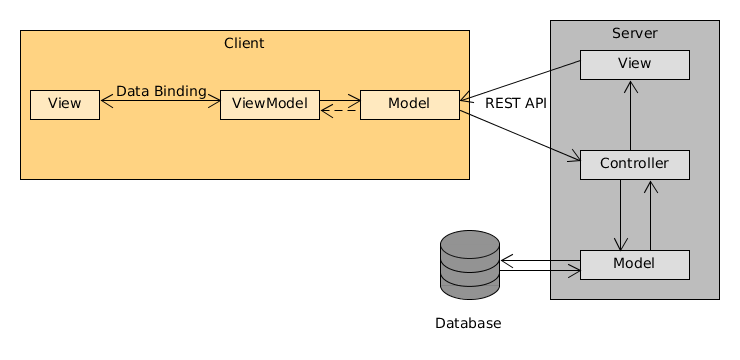
\includegraphics[scale = .6]{systemarchitektur.png}
    		\caption{Systemarchitektur}
    	\end{figure}
    
    	Die Systemarchitektur der App trennt sich in die Server- und die Client-Seite mit dem REST (Representational State Transfer) Architektur-Stil. Dabei stellt der Server einen Dienst bereit, der bei Bedarf vom Client durch die Verwendung von HTTP-Methoden angefragt werden kann. \\
    	Die Client-Seite verwendet das MVVM (Model-View-ViewModel) Architektur-Muster mit Datenbindung. Auf der Server-Seite wird das MVC (Model-View-Controller) Architektur-Muster eingesetzt.
    	
    
    	\clearpage
    		
        \section{Szenarien}
        
        
        \subsection{Was mache ich mit meinem Kuchen?}
        Max Mustermann wohnt seit 2016 in einer WG. Am Wochenende hatte er Geburtstag und hat von zu Hause Kuchen mitgebracht. In einer großen Dose sind Stücke von seinem Lieblings-Schokokuchen und auch Zitronenkuchen. Er will die Dose nicht in das Gemeinschaftsfach im Kühlschrank legen, da er für sich und seine Freundin den Schokokuchen behalten möchte, aber er möchte nicht noch mal zwei Dosen beschmutzen, um die zwei Sorten zu teilen.\\
        Dann erinnert er sich daran, dass, als er mit seinen Kumpels die WG gegründet hat, einer seiner Mitbewohner die WG mit Fridget bekanntgemacht hat. Er kann jetzt in der App eine neue  erstellen, mit der Überschrift ``Kuchen!“, in der er allen seinen Mitbewohnern mitteilen kann, dass es Kuchen zum Essen gibt, aber spezifizieren kann, was gegessen und was übrig bleiben soll. Er kann außerdem durch die Lesebestätigungen sehen, dass alle seine Mitbewohner die Notiz gelesen haben.
        \\
        
        \subsection{Medizinischer Notfall}
        Hannah Schmidt ist schon im vierten Semester ihres Studiums und hat endlich eine WG in Laufdistanz zur Uni gefunden. Sie lernt ihre Mitbewohner einen nach dem anderen kennen und erfährt, dass einer ihrer Mitbewohner eine schwere Allergie hat. Dann fällt ihr ein, wie viele Schwierigkeiten sie hatte, mit den Eltern Kontakt aufzunehmen, als ihre ehemalige Mitbewohnerin einen schweren Unfall hatte.\\
        Zum Glück gibt es bei Fridget eine Möglichkeit, durch \textit{Frozen Notes} Notfallkontakte immer zur Hand zu haben. Die \textit{Frozen Notes} sind fest, nicht löschbar und klar sichtbar in der App. Hannah lädt die App herunter und registriert sich mit ihrem Google Account. Dann kann sie eine WG-Pinnwand mit einem einzigartigen Zugangscode generieren und ihre Mitbewohner können damit auf genau diese WG-Pinnwand zugreifen. Hannah empfiehlt dann jedem ihrer Mitbewohner, seine Notfallkontakte hineinzuschreiben, sodass diese immer verfügbar sind, ohne danach suchen oder fragen zu müssen.
        \newpage
        
        \subsection{Ankündigungen}
        Mia wohnt mit ihrem Freund Hans in einer Wohnung zusammen. Als sie nach der Arbeit zu Hause ankommt, merkt sie, dass der Hausmeister mehrere Ankündigungen an ihre Haustür geklebt hat, unter anderem einen Zettel mit den Daten der Altpapiersammlung.
        Anstatt diese ganzen Ankündigungen auf Papier kopieren zu müssen, macht Mia Bilder von den Zetteln. Die Bilder kann sie dann mit einer Beschreibung auf die Pinnwand hochladen, damit Mia und Hans beide jederzeit die Bilder zur Verfügung haben.
        

        \newpage
			\documentclass[a4paper]{scrreprt}
\usepackage[german]{babel}
\usepackage[utf8]{inputenc}
\usepackage[T1]{fontenc}
\usepackage{graphicx}
\graphicspath{ {images/} }
\usepackage{ae}

\begin{document}
    \chapter{Anwendungsfälle}
    		\begin{figure}[h]
			\centering
			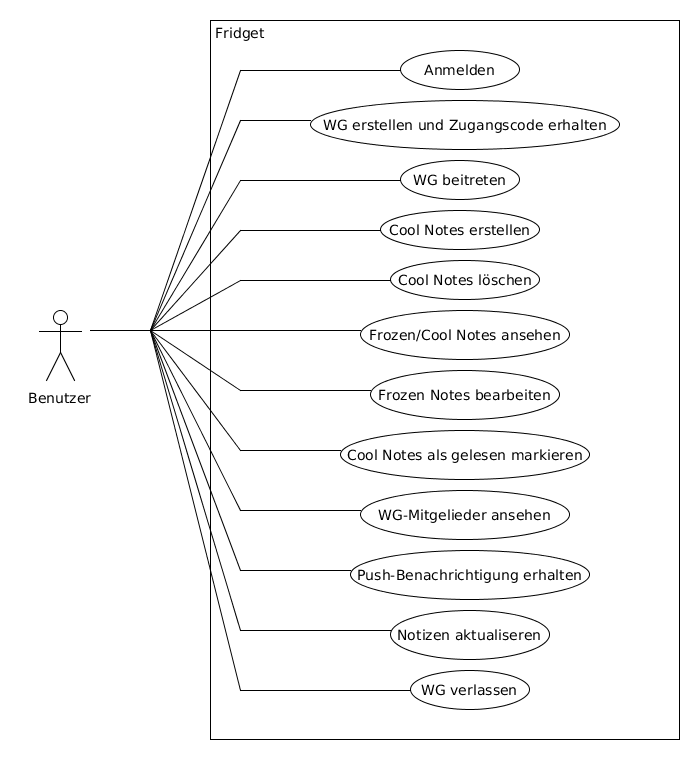
\includegraphics[scale = .6]{anwendungsfalldiagramm.png}
			\caption{Anwendungsfalldiagramm}
		\end{figure}
    		    		
        \section{Anmelden}
        \textbf{Teilnehmende Akteure}: Benutzer \\
		\textbf{Eingangsbedingungen}: Der Benutzer hat Fridget installiert und besitzt ein Google-Konto. Das Internet ist verfügbar. \\
		\textbf{Ausgangsbedingung}: Der Benutzer hat sich angemeldet. \\
		\textbf{Ereignisfluss}: Benutzer wird angemeldet
		
		\section{WG erstellen und Zugangscode erhalten}
		\textbf{Teilnehmende Akteure}: Benutzer \\
		\textbf{Eingangsbedingungen}: Der Benutzer hat sich angemeldet. Das Internet ist verfügbar. \\
		\textbf{Ausgangsbedingung}: Ein Zugangscode wurde angezeigt. \\
		\textbf{Ereignisfluss}: WG wird erstellt $\rightarrow$ Zugangscode wird generiert
		
		\section{WG beitreten}
		\textbf{Teilnehmende Akteure}: Benutzer \\
		\textbf{Eingangsbedingungen}: Der Benutzer hat sich angemeldet und besitzt einen gültigen Zugangscode. Die WG ist nicht voll. Das Internet ist verfügbar. \\
		\textbf{Ausgangsbedingung}: Der Benutzer ist einer WG beigetreten. \\
		\textbf{Ereignisfluss}: WG wird beigetreten
		
		\section{Cool Notes erstellen}
		\textbf{Teilnehmende Akteure}: Benutzer \\
		\textbf{Eingangsbedingungen}: Der Benutzer hat sich angemeldet und ist einer WG beigetreten. Die Pinnwand ist nicht voll und keiner erstellt gerade die letzte Cool Note. Das Internet ist verfügbar. \\
		\textbf{Ausgangsbedingung}: Der Benutzer hat das Erstellen bestätigt. \\
		\textbf{Ereignisfluss}: Cool Note wird erstellt
		
		\section{Cool Notes löschen}
		\textbf{Teilnehmende Akteure}: Benutzer \\
		\textbf{Eingangsbedingungen}: Der Benutzer hat eine Cool Note, die nicht von ihm erstellt wurde, geöffnet. Keiner liest gerade dieselbe Cool Note. Das Internet ist verfügbar. \\
		\textbf{Ausgangsbedingung}: Der Benutzer hat das Löschen bestätigt. \\
		\textbf{Ereignisfluss}: Cool Note wird gelöscht
		
		\section{Frozen/Cool Notes ansehen}
		\textbf{Teilnehmende Akteure}: Benutzer \\
		\textbf{Eingangsbedingungen}: Der Benutzer hat sich angemeldet und ist einer WG beigetreten. Die Pinnwand ist nicht leer. Das Internet ist verfügbar. \\
		\textbf{Ausgangsbedingung}: Eine Frozen/Cool Note wurde angezeigt. \\
		\textbf{Ereignisfluss}: Frozen/Cool Note wird geöffnet $\rightarrow$ Frozen/Cool Note wird angesehen
		
		\section{Frozen Notes bearbeiten}
		\textbf{Teilnehmende Akteure}: Benutzer \\
		\textbf{Eingangsbedingungen}: Der Benutzer hat eine Frozen Note geöffnet. Keiner bearbeitet gerade dieselbe Frozen Note. Das Internet ist verfügbar. \\
		\textbf{Ausgangsbedingung}: Der Benutzer hat das Bearbeiten bestätigt. \\
		\textbf{Ereignisfluss}: Frozen Note wird bearbeitet
		
		\section{Cool Notes als gelesen markieren}
		\textbf{Teilnehmende Akteure}: Benutzer \\
		\textbf{Eingangsbedingungen}: Der Benutzer hat eine Cool Note, die nicht von ihm erstellt wurde, geöffnet. Die Cool Note wurde noch nicht als gelesen markiert. Das Internet ist verfügbar. \\
		\textbf{Ausgangsbedingung}: Der Benutzer hat die Cool Note als gelesen markiert. \\
		\textbf{Ereignisfluss}: Cool Note wird markiert
		
		\section{WG-Mitgelieder ansehen}
		\textbf{Teilnehmende Akteure}: Benutzer \\
		\textbf{Eingangsbedingungen}: Der Benutzer hat sich angemeldet und ist einer WG beigetreten. Das Internet ist verfügbar. \\
		\textbf{Ausgangsbedingung}: Die WG-Mitgelieder werden angezeigt. \\
		\textbf{Ereignisfluss}: WG-Mitgelieder-View wird geöffnet $\rightarrow$ WG-Mitgelieder werden angesehen
		
		\section{Push-Benachrichtigung erhalten}
		\textbf{Teilnehmende Akteure}: Benutzer \\
		\textbf{Eingangsbedingungen}: Der Benutzer hat sich angemeldet und ist einer WG beigetreten. Der Benutzer hat ``Push-Benachrichtigung'' von Fridget aktiviert. Das Internet ist verfügbar. \\
		\textbf{Ausgangsbedingung}: Die Push-Benachrichtigung wird auf den Geräten des Benutzers angezeigt. \\
		\textbf{Ereignisfluss}: Neue Cool Note wird erstellt $\rightarrow$ Push-Benachrichtigung wird erhalten
		
		\section{Notizen/Mitglieder aktualisieren}
		\textbf{Teilnehmende Akteure}: Benutzer \\
		\textbf{Eingangsbedingungen}: Der Benutzer hat sich angemeldet und ist einer WG beigetreten. Das Internet ist verfügbar. \\
		\textbf{Ausgangsbedingung}: Die Änderungen von Notizen/Mitgliedern wurden mit dem Server synchronisiert. \\
		\textbf{Ereignisfluss}: Pinnwand wird nach unten gewischt $\rightarrow$ Notizen/Mitglieder werden aktualisiert
		
		\section{WG verlassen}
		\textbf{Teilnehmende Akteure}: Benutzer \\
		\textbf{Eingangsbedingungen}: Der Benutzer hat sich angemeldet und ist einer WG beigetreten. Das Internet ist verfügbar. \\
		\textbf{Ausgangsbedingung}: Der Benutzer hat das Verlassen der WG bestätigt. \\
		\textbf{Ereignisfluss}: WG wird verlassen
\end{document}
        	
        	\newpage
        \section{Bedienoberfläche}
        
        \begin{figure}[h]
        	\begin{minipage}[b]{0.4\linewidth}
        		
        		\flushright
        		\centering
        		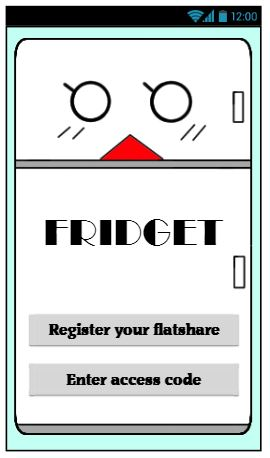
\includegraphics[width=0.7\textwidth]{fridget_start.JPG}
        		\caption{Startbildschirm}
        		\label{fig:figure1}
        	\end{minipage}
        	\hspace{0.5cm}
        	\begin{minipage}[b]{0.55\linewidth}
        		\flushleft
        		{[}S01{]} Startbildschirm \\
        		\hfill
        		\\Beschreibung: \\
        		Startbildschirm der App. Dieser erscheint nachdem man sich mit dem Google-Account angemeldet hat. Man hat die Wahl zwischen WG erstellen und Zugangscode eingeben, um einer bereits vorhandenen WG beizutreten.
        		\\
        		\hfill 
        		\\Elemente:
        		\begin{itemize}
        		\renewcommand\labelitemi{--}
        		\item Button zum Erstellen der WG
        		\item Button zum Eingeben des Zugangscodes
        		\end{itemize}
        	
        		\hfill
        		
        		Verwendung:\\
        		Durch das Tippen auf den oberen Button
        		kann man eine WG erstellen, indem man ihr
        		einen Namen gibt {[}S02{]}.\\
        		Durch das Tippen auf den unteren Button kann
        		man den Zugangscode eingeben {[}S04{]}, den man zuvor vom WG-Ersteller extern erhalten 
        		hat.
        		
        	\end{minipage}
        \end{figure}
    
    	\begin{figure}[h!]
    		\begin{minipage}[t]{0.4\linewidth}
    			\flushright
    			\centering
    			\vspace{9mm}
    			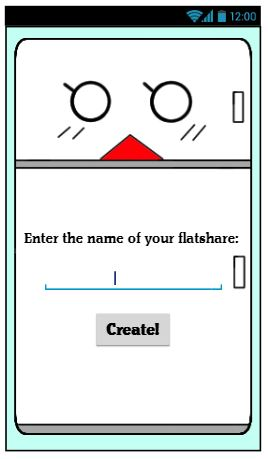
\includegraphics[width=0.7\textwidth]{fridget_nameenter.JPG}
    			\caption{Namensgebung}
    			\label{fig:figure1}
    		\end{minipage}
    		\hspace{0.5cm}
    		\begin{minipage}[t]{0.55\linewidth}
    			\flushleft
    			\vspace{9mm}
    			{[}S02{]} Namensgebung\\
    			\hfill
    			\\Beschreibung: \\
    			View zur Namesgebung einer WG.\\
    			\hfill
    			\\Elemente:
    			\begin{itemize}
    				\renewcommand\labelitemi{--}
    				\item Textfeld zum Eingeben des Namens
    				\item Button zum endgültigen Erstellen der WG
    				
    			\end{itemize}
    		
    			\hfill
    			
    			Verwendung:\\
    			Durch das Tippen auf das Textfeld kann man
    			den Namen der WG eingeben. \\
    			Durch das Tippen auf den Button wird ein 
    			zufälliger aber einzigartiger Zugangscode 
    			generiert und ausgegeben {[}S03{]}.
    			
    			
    			
    		\end{minipage}
    	\end{figure}
    
    	\clearpage
    	
    	\begin{figure}[h]
    		\begin{minipage}[b]{0.4\linewidth}
    			
    			\flushright
    			\centering
    			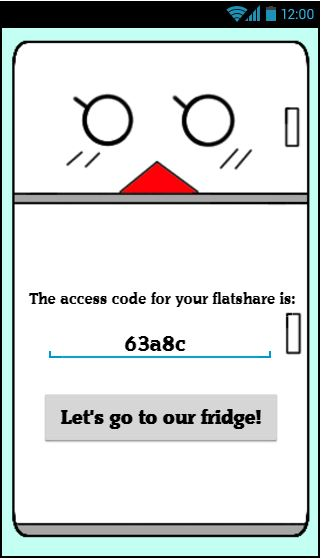
\includegraphics[width=0.7\textwidth]{fridget_accesscode.JPG}
    			\caption{Zugangscode bekommen}
    			\label{fig:figure1}
    			\vspace{13mm}
    		\end{minipage}
    		\hspace{0.5cm}
    		\begin{minipage}[b]{0.55\linewidth}
    			\flushleft
    			
    			{[}S03{]} Zugangscode bekommen \\
    			\hfill
    			\\Beschreibung: \\
    			View zum Erhalten des Zugangscodes.\\
    			\hfill
    			\\Elemente:
    			\begin{itemize}
    				\renewcommand\labelitemi{--}
    				\item Textfeld für die Ausgabe des Zugangscodes
    				\item Button zum Gelangen zur WG-Pinnwand
    				
    			\end{itemize}
    		
    			\hfill
    			
    			Verwendung:\\
    			Durch das Tippen auf den Button gelangt man
    			zur erstellten WG-Pinnwand. {[}S05{]}.
    			
    			\vspace{38mm}
    			
    		\end{minipage}
    	\end{figure}
    	
    	\begin{figure}[h!]
    		\begin{minipage}[t]{0.4\linewidth}
    			\flushright
    			\centering
    			\vspace{9mm}
    			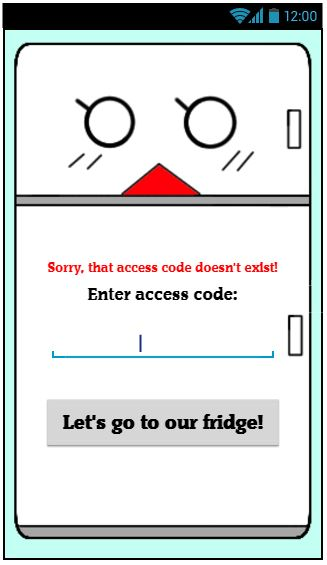
\includegraphics[width=0.7\textwidth]{fridget_accesscodeenter.JPG}
    			\caption{Zugangscode eingeben}
    			\label{fig:figure1}
    		\end{minipage}
    		\hspace{0.5cm}
    		\begin{minipage}[t]{0.55\linewidth}
    			\flushleft
    			\vspace{9mm}
    			{[}S04{]} Zugangscode eingeben \\
    			\hfill
    			\\Beschreibung: \\
    			View zum Eingeben des Zugangscodes.\\
    			\hfill
    			\\Elemente:
    			\begin{itemize}
    				\renewcommand\labelitemi{--}
    				\item Textfeld zur Eingabe des Zugangscodes
    				\item Button zum Gelangen zur WG-Pinnwand
    				\item Fehlermeldung bei falscher Eingabe
    			\end{itemize}
    		
    			\hfill
    			
    			Verwendung:\\
    			Durch das Tippen auf das Textfeld kann man
    			den Zugangscode eingeben. Falls dieser falsch 
    			ist, erscheint die Fehlermeldung in Rot.
    			\\
    			Durch das Tippen auf den Button gelangt man
    			zur erstellten WG-Pinnwand. {[}S05{]}. 
    			
    			
    			
    		\end{minipage}
    	\end{figure}
    
    	\clearpage
    	
    	\begin{figure}[h]
    		\begin{minipage}[b]{0.4\linewidth}
    			
    			\flushright
    			\centering
    			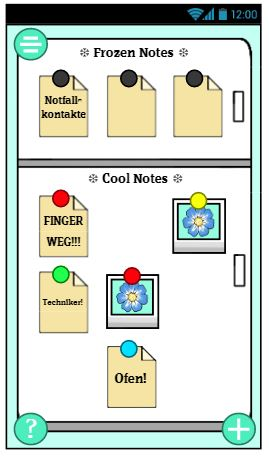
\includegraphics[width=0.7\textwidth]{fridget_fridge.JPG}
    			\caption{WG-Pinnwand}
    			\label{fig:figure1}
    			\vspace{8cm}
    		\end{minipage}
    		\hspace{0.5cm}
    		\begin{minipage}[b]{0.55\linewidth}
    			\flushleft
    			{[}S05{]} WG-Pinnwand \\
    			\hfill
    			\\Beschreibung: \\
    			View der WG-Pinnwand, man sieht die Notes mit Überschrift und Magnet und einige Buttons. \\ Drei Frozen Notes sind von Anfang an enthalten. Frozen Notes haben immer einen schwarzen Magneten.
    			\\
    			\hfill
    			\\Elemente:
    			\begin{itemize}
    				\renewcommand\labelitemi{--}
    				\item  Drei fixed \textit{Frozen Notes}
    				\item Ein paar \textit{Cool Notes} (Text und Bild)
    				\item Menü-Button {[}B01{]} für das Menü (links oben)
    				\item Hilfe-Button {[}B08{]} für das Tutorial (links unten)
    				\item Plus-Button {[}B04{]} zum Erstellen einer \textit{Cool Note}
    				(rechts unten)
    				
    			\end{itemize}
    			
    			\hfill
    			
    			Verwendung:\\
    			Durch das Tippen auf eine Frozen oder Cool
    			Note gelangt man in die Großansicht {[}S06{]}.
    			\\
    			Durch das Tippen auf den Menü-Button {[}B01{]} 
    			öffnet sich das Menü {[}S07{]}.\\
    			Durch das Tippen auf den Hilfe-Button  {[}B08{]} erscheint
    			ein Tutorial-Overlay {[}S16{]} auf der Pinnwand.	\\
    			Durch das Tippen auf den  Plus-Button [B04]  erscheint 
    			ein Pop-Up zur Entscheidung {[}S08{]}, welche Art von Cool Note man erstellen möchte (Text oder
    			Bild).\\
    			Durch Hinunterswipen kann man manuell aktualisieren.
    			
    		\end{minipage}
    	\end{figure}
    	
    	
    
    	
    	
    	
    	
    	\clearpage
    	
    	\begin{figure}[h]
    		\begin{minipage}[b]{0.4\linewidth}
    			
    			\flushright
    			\centering
    			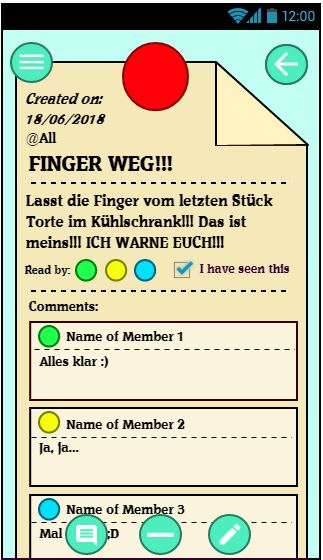
\includegraphics[width=0.7\textwidth]{fridget_notebig.JPG}
    			\caption{Großansicht einer Textnotiz}
    			\label{fig:figure1}
    			\vspace{13cm}
    		\end{minipage}
    		\hspace{0.5cm}
    		\begin{minipage}[b]{0.55\linewidth}
    			\flushleft
    			{[}S06{]} Großansicht einer Textnotiz \\
    			\hfill
    			\\Beschreibung: \\
    			Großansicht einer Note mit zugehörigen Magnet  (bei einer \textit{Frozen Note} wäre dieser schwarz), Erstelldatum, Tags, Titel, Inhalt, Lesebestätigungen und Kommentaren. Der @All-Tag ist immer da, wenn keine Tags spezifiziert werden. Man sieht außerdem wieder einige Buttons, der Edit-Button {[}B05{]} ist nur bei \textit{Frozen Notes} sichtbar. Der Minus-Button {[}B03{]}  und Kommentar-Button {[}B06{]} ist nur bei seinen eigenen \textit{Cool Notes} sichtbar. Die Anzeige der Tags und die Lesebestätigungen sind auch nur bei \textit{Cool Notes} sichtbar. Bei diesem View kann man scrollen.
    			\\
    			\hfill
    			\\Elemente:\\
    			\begin{itemize}
    				\renewcommand\labelitemi{--}
    				\item  Menü-Button {[}B01{]} für das Menü ({[}S07{]}).
    				\item Zurück-Button {[}B02{]} zum Gelangen zur
    				WG-Pinnwand-Ansicht {[}S05{]}.
    				\item Kommentar-Button {[}B06{]} zum Erstellen eines
    				Kommentars.
    				\item Minus-Button {[}B03{]} zum Löschen der Note.
    				\item Edit-Button {[}B05{]} zum Editieren der Note.
    				\item Checkbox zum Abhaken, ob man die Note gelesen hat oder nicht.
    				
    			\end{itemize}
    			
    			\hfill
    			
    			Verwendung:\\
    			Man kann den Inhalt der Note lesen und durch
    			das Tippen des Kommentar-Buttons {[}B06{]}
    			kommentieren. \\
    			Durch das Tippen auf den 
    			Minus-Button {[}B03{]} erscheint ein Pop-Up, das abfragt, ob man die Note wirklich löschen möchte {[}S08{]}.\\
    			Durch das Tippen des Edit-Buttons {[}B05{]} erscheint
    			dasselbe View wie beim Erstellen einer Note {[}S10{]}, nur ohne die Auswahl der Wichtigkeit.\\ Durch Antippen der Checkbox kann man für sich Markieren, ob man die Note gesehen hat oder nicht.\\
    			Durch Hinunterswipen kann man die Note aktualisieren.
    			
    		\end{minipage}
    	\end{figure}
    	
    	\clearpage
    	
    	\begin{figure}[h]
    		\begin{minipage}[b]{0.4\linewidth}
    			\flushright
    			\centering
    			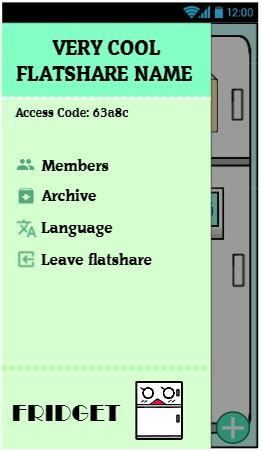
\includegraphics[width=0.7\textwidth]{fridget_menu.JPG}
    			\caption{Menü}
    			\label{fig:figure1}
    			\vspace{20mm}
    		\end{minipage}
    		\hspace{0.5cm}
    		\begin{minipage}[b]{0.55\linewidth}
    			\flushleft
    			{[}S07{]} Menü \\
    			\hfill
    			\\Beschreibung: \\
    			Menü mit WG-Namen, Zugangscode und
    			Menüpunkte für Profil, Mitglieder, Archiv,
    			Sprache und WG verlassen. Ganz unten ist das
    			Fridget Logo.\\
    			
    			\hfill 
    			\\Elemente:
    			\begin{itemize}
    				\renewcommand\labelitemi{--}
    				\item Menüpunkt ``Members”
    				\item Menüpunkt ``Archive”
    				\item Menüpunkt ``Language”
    				\item Menüpunkt ``Leave flatshare”
    				
    			\end{itemize}
    		
	    		\hfill
	    		\\
    			
    			Verwendung:\\
    			Durch das Tippen auf den Menüpunkt
    			``Members” öffnet sich das Members-View {[}S11{]}
    			Menüpunkte öffnen sich die Menü-Views {[}S12{]}.\\ Durch das Swipen des Menüs nach links wird diese wieder geschlossen und man sieht die Kühlschrank-View {[}S05{]}.
    			
    			\vspace{1mm}
    			
    		\end{minipage}
    	\end{figure}
    	
    	\begin{figure}[h!]
    		\begin{minipage}[t]{0.4\linewidth}
    			\flushright
    			\centering
    			\vspace{9mm}
    			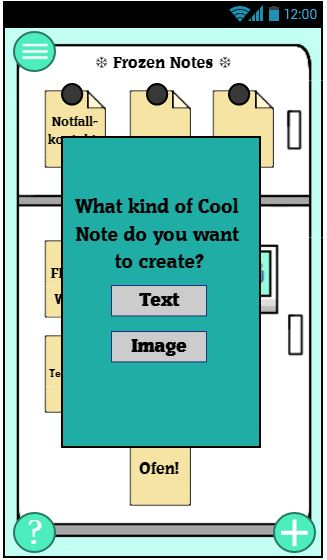
\includegraphics[width=0.7\textwidth]{fridget_type.JPG}
    			\caption{Pop-Ups mit Abfrage}
    			\label{fig:figure1}
    		\end{minipage}
    		\hspace{0.5cm}
    		\begin{minipage}[t]{0.55\linewidth}
    			\flushleft
    			\vspace{9mm}
    			{[}S08{]} Pop-Ups mit Abfrage \\
    			\hfill
    			\\
    			Beschreibung: \\
    			Pop-Up mit Abfrage und Buttons. 
    			\\
    			Elemente:\\
    			Buttons mit jeweiligen Antwortmöglichkeiten.\\
    			
    			\hfill 
    			
    			Verwendung:\\
    			 Dienen zur Sicherheitsabfrage und genereller 
    			Entscheidungsabfrage.\\ Durch das Tippen auf
    			einen Button öffnet sich das jeweilige View oder
    			das Pop-Up verschwindet oder es öffnet sich ein
    			Pop-Up ohne Abfrage.
    			 
    			
    			
    			
    		\end{minipage}
    	\end{figure}
    	
    	\clearpage
    	
    	\begin{figure}[h!]
    		\begin{minipage}[t]{0.45\linewidth}
    			\flushright
    			\centering
    			\vspace{9mm}
    			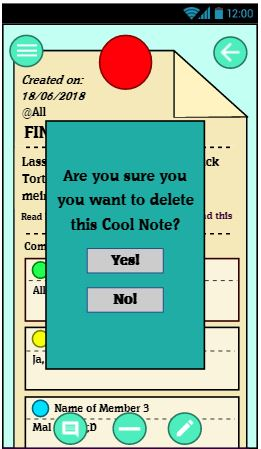
\includegraphics[width=0.6\textwidth]{fridget_delete.JPG}
    			\caption{Pop-Ups mit Abfrage}
    			\label{fig:figure1}
    		\end{minipage}
    		\hspace{0.5cm}
    		\begin{minipage}[t]{0.45\linewidth}
    			\flushright
    			\centering
    			\vspace{9mm}
    			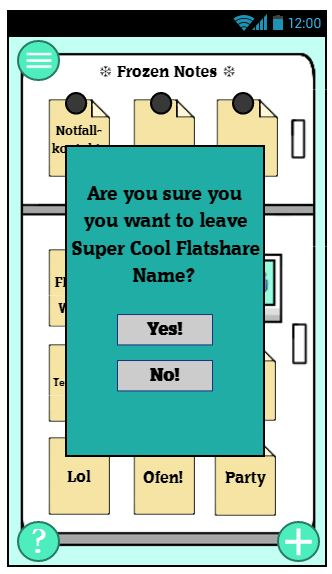
\includegraphics[width=0.6\textwidth]{fridget_leave.JPG}
    			\caption{Pop-Ups mit Abfrage}
    			\label{fig:figure1}
    			
    		\end{minipage}
    	\end{figure}
    
    	\vspace{15mm}
    	
    	\begin{figure}[h!]
    		\begin{minipage}[b]{0.4\linewidth}
    			\flushright
    			\centering
    			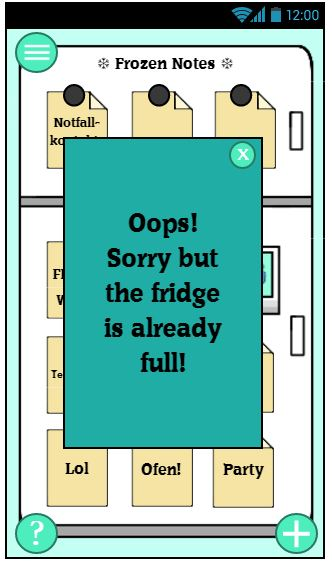
\includegraphics[width=0.7\textwidth]{fridget_error.JPG}
    			\caption{Pop-Ups ohne Abfrage}
    			\label{fig:figure1}
    			\vspace{1mm}
    		\end{minipage}
    		\hspace{0.5cm}
    		\begin{minipage}[b]{0.55\linewidth}
    			\flushleft
    			{[}S09{]} Pop-Ups ohne Abfrage\\
    			\hfill
    			\\Beschreibung: \\
    			Pop-Up ohne Abfrage mit Close-Button.\\
    			
    			\hfill 
    			\\Elemente:\\
    			Close-Button (rechts oben beim Popup) zum 
    			Schließen des Pop-Ups.\\
    			
    				
    			
    			\hfill
    			\\
    			
    			Verwendung:\\
    			Dienen hauptsächlich zum Anzeigen von
    			Fehlermeldungen und anderweitigen
    			Mitteilungen der App. Durch das Antippen des 
    			Close-Buttons wird das Pop-Up geschlossen.
    			
    			
    			\vspace{17mm}
    			
    		\end{minipage}
    	\end{figure}
    	
    	\clearpage
    	
    	\begin{figure}[h!]
    		\begin{minipage}[t]{0.4\linewidth}
    			\flushright
    			\centering
    			\vspace{9mm}
    			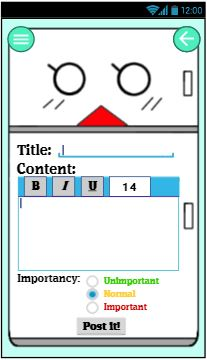
\includegraphics[width=0.7\textwidth]{fridget_textnote.JPG}
    			\caption{Textnotiz}
    			\label{fig:figure1}
    		\end{minipage}
    		\hspace{0.5cm}
    		\begin{minipage}[t]{0.55\linewidth}
    			\flushleft
    			\vspace{9mm}
    			{[}S10{]} Textnotiz \\
    			\hfill
    			\\
    			Beschreibung: \\
    			View für die Bearbeitung einer Cool Note mit
    			Text.
    			 
    			\hfill 
    			\\Elemente:\\
    			\begin{itemize}
    				\renewcommand\labelitemi{--}
    				\item  Hamburger-Button für das Menü ({[}S07{]})
    				\item Textfeld zum Eingeben der Notiz-Überschrift
    				\item Edit-Bar zum Bearbeiten des Textes (Bold,
    				Italic, Underline)
    				\item Radio Buttons zum Einstellen der Wichtigkeit 
    				der Notiz
    				\item Button zum Posten der \textit{Cool Note}
    				\item Zurück-Button zum Gelangen zur
    				WG-Pinnwand-Ansicht {[}S05{]} und Abbrechen des Notiz-Erstellens.
    				
    			\end{itemize}
    			
    			
    			\hfill 
    			
    			Verwendung:\\
    			Durch das Tippen auf die Textfelder kann 
    			der Text geschrieben werden.\\
    			Durch das
    			Antippen der Radio-Buttons kann die 
    			Wichtigkeit ausgewählt werden. Ist man 
    			fertig, wird durch das Antippen des Buttons
    			die Notiz erstellt und  in der
    			Kühlschrank-View {[}S05{]} sichtbar.\\ 
    			Zum
    			Taggen schreibt man @NamedesMitglieds  
    			in das Content-Feld.
    			
    			
    			
    		\end{minipage}
    	\end{figure}
    	
    	\clearpage
    	
    	\begin{figure}[h]
    		\begin{minipage}[b]{0.35\linewidth}
    			\flushright
    			\centering
    			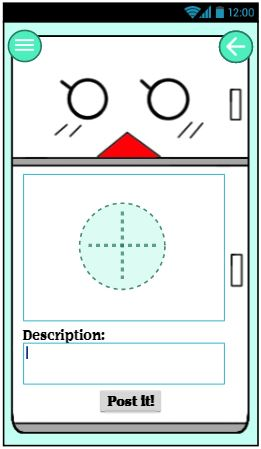
\includegraphics[width=0.7\textwidth]{fridget_picnote.JPG}
    			\caption{Bildnotiz}
    			\label{fig:figure1}
    			\vspace{43mm}
    		\end{minipage}
    		\hspace{0.5cm}
    		\begin{minipage}[b]{0.65\linewidth}
    			\flushleft
    			{[}S11{]} Bildnotiz \\
    			\hfill
    			\\Beschreibung: \\
    			View für die Bearbeitung einer Cool Note mit
    			Bild.\\
    			
    			\hfill 
    			\\Elemente:
    			\begin{itemize}
    				\renewcommand\labelitemi{--}
    				\item Hamburger-Button für das Menü ({[}S07{]})
    				\item Plus-Button zum Hochladen einer Bild-Datei
    				\item Textfeld zum Eingeben einer Beschreibung des 
    				Bildes
    				\item Button zum Posten des Bildes
    				\item Zurück-Button zum Gelangen zur
    				WG-Pinnwand-Ansicht {[}S05{]} und Abbrechen des Notiz-Erstellens.
    				
    			\end{itemize}
    			
    			\hfill
    			\\
    			
    			Verwendung:\\
    			Durch das Tippen auf den Plus-Button öffnet 
    			sich das lokale Datenverzeichnis des Handys 
    			zum Auswählen einer Bilddatei. Eine Vorschau 
    			des Bildes wird dann im Kasten sichtbar.\\ 
    			Durch
    			das Antippen des Textfeldes kann eine
    			Beschreibung zum Bild geschrieben werden. Ist
    			man fertig, wird durch das Antippen des Buttons  
    			die Notiz erstellt und in der Kühlschrank-View 
    			{[}S05{]} sichtbar. 
    			
    			\vspace{1mm}
    			
    		\end{minipage}
    	\end{figure}
    	
    	\begin{figure}[h!]
    		\begin{minipage}[t]{0.35\linewidth}
    			\flushright
    			\centering
    			\vspace{9mm}
    			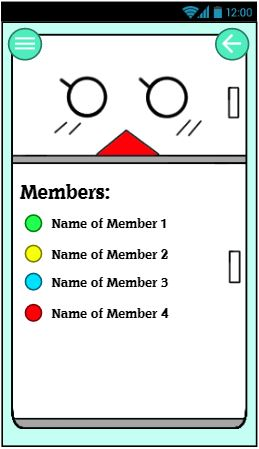
\includegraphics[width=0.7\textwidth]{fridget_members.JPG}
    			\caption{Mitglieder}
    			\label{fig:figure1}
    		\end{minipage}
    		\hspace{0.5cm}
    		\begin{minipage}[t]{0.65\linewidth}
    			\flushleft
    			\vspace{9mm}
    			{[}S12{]} Mitglieder \\
    			\hfill
    			\\
    			Beschreibung: \\
    			View zum Einsehen der aktuellen Mitglieder mit
    			mit zugehörigem Magnet.\\
    			\hfill
    			Elemente:\\
    			\begin{itemize}
    				\renewcommand\labelitemi{--}
    				\item Hamburger-Button für das Menü ({[}S07{]})
    				\item Magnete mit Mitgliedernamen nebendran.
    				Die Namen werden vom Google-Account
    				ausgelesen
    				\item Zurück-Button zum Gelangen zur
    				WG-Pinnwand-Ansicht {[}S05{]}.
    				
    			\end{itemize}
    			
    			\hfill 
    			
    			Verwendung:\\
    			Durch das Tippen auf die Namen kommt man 
    			zum Profil des jeweiligen Mitglieds.
    			   			
    			
    		\end{minipage}
    	\end{figure}
    	\clearpage
    	
    	\begin{figure}[h]
    		\begin{minipage}[b]{0.37\linewidth}
    			\flushright
    			\centering
    			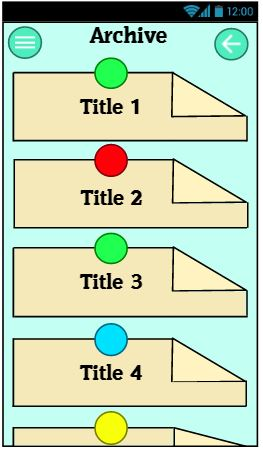
\includegraphics[width=0.7\textwidth]{fridget_archive.JPG}
    			\caption{Archiv}
    			\label{fig:figure1}
    			\vspace{22mm}
    		\end{minipage}
    		\hspace{0.5cm}
    		\begin{minipage}[b]{0.6\linewidth}
    			\flushleft
    			{[}S13{]} Archive \\
    			\hfill
    			\\Beschreibung: \\
    			View zum Einsehen der archivierten \textit{Cool Notes}.
    			Man sieht die Notes mit Magnet und Überschrift.
    			Bei diesem View kann man scrollen.\\
    			
    			\hfill 
    			\\Elemente:
    			\begin{itemize}
    				\renewcommand\labelitemi{--}
    				\item Hamburger-Button für das Menü ({[}S07{]})
    				\item \textit{Cool Notes} mit Magnet und Überschrift
    				\item Zurück-Button zum Gelangen zur
    				WG-Pinnwand-Ansicht {[}S05{]}.
    				
    			\end{itemize}
    			
    			\hfill
    			\\
    			
    			Verwendung:\\
    			Durch das Tippen auf die archivierten Cool Notes
    			kann man die Großansicht der entsprechenden
    			Notes ansehen {[}S06{]}.
    			
    			\vspace{20mm}
    			
    		\end{minipage}
    	\end{figure}
    	
    	\begin{figure}[h!]
    		\begin{minipage}[t]{0.37\linewidth}
    			\flushright
    			\centering
    			\vspace{1mm}
    			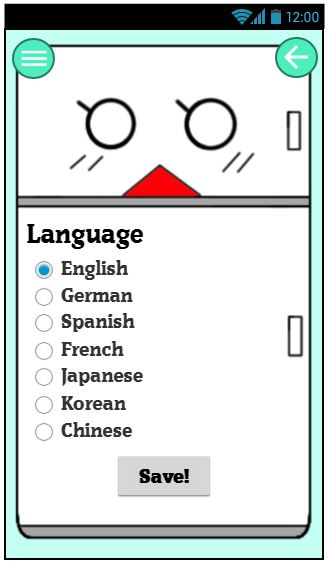
\includegraphics[width=0.7\textwidth]{fridget_language.JPG}
    			\caption{Sprache}
    			\label{fig:figure1}
    			\vspace{15mm}
    		\end{minipage}
    		\hspace{0.5cm}
    		\begin{minipage}[t]{0.6\linewidth}
    			\flushleft
    			{[}S14{]} Sprache \\
    			\hfill
    			\\
    			Beschreibung: \\
    			View zum Einstellen der App-Sprache.\\
    			
    			\hfill
    			\\Elemente:\\
    			\begin{itemize}
    				\renewcommand\labelitemi{--}
    				\item Hamburger-Button für das Menü ({[}S07{]})
    				\item Radio-Buttons zum Einstellen der App-Sprache
    				\item Save-Button zum Speichern der Änderungen
    				\item Zurück-Button zum Gelangen zur
    				WG-Pinnwand-Ansicht {[}S05{]}.
    				
    			\end{itemize}
    			
    			\hfill 
    			
    			Verwendung:\\
    			Durch das Tippen auf einen der jeweiligen
    			Radio-Buttons kann man eine andere Sprache
    			auswählen.\\
    			Durch das Tippen auf den
    			Save-Button werden die Änderungen
    			gespeichert.
    			
    			
    		\end{minipage}
    	\end{figure}
    	
    	\clearpage
    	
    	\begin{figure}[h!]
    		\begin{minipage}[t]{0.4\linewidth}
    			\flushright
    			\centering
    			\vspace{9mm}
    			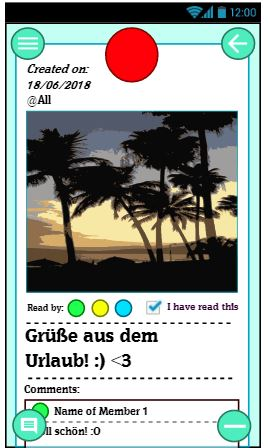
\includegraphics[width=0.7\textwidth]{fridget_picnotebig.JPG}
    			\caption{Großansichet einer Bildnotiz}
    			\label{fig:figure1}
    		\end{minipage}
    		\hspace{0.5cm}
    		\begin{minipage}[t]{0.55\linewidth}
    			\flushleft
    			\vspace{9mm}
    			{[}S15{]} Großansicht einer Bildnotiz \\
    			\hfill
    			\\
    			Beschreibung: \\
    			Großansicht einer Bild-Notiz mit zugehörigen Magnet, Erstelldatum, Tags, Lesebestätigungen, Beschreibung und Kommentaren. Der @All-Tag ist immer da, wenn keine Tags spezifiziert werden. Man sieht außerdem wieder einige Buttons. Bei diesem View kann man scrollen.
    			
    			\hfill 
    			\\Elemente:\\
    			\begin{itemize}
    				\renewcommand\labelitemi{--}
    				\item  Hamburger-Button für das Menü ({[}S07{]})
    				\item Zurück-Button zum Gelangen zur
    				WG-Pinnwand-Ansicht {[}S05{]}.
    				\item Kommentar-Button zum Erstellen eines
    				Kommentars.
    				\item Minus-Button zum Löschen der Note.
    				\item Checkbox zum Abhaken, ob man die Note gelesen hat oder nicht.
    				
    			\end{itemize}
    			
    			
    			\hfill 
    			
    			Verwendung:\\
    			Man kann das Bild und den Inhalt der
    			Beschreibung der Note lesen und durch
    			das Tippen des Kommentar-Buttons
    			kommentieren. \\
    			Durch das Tippen auf den 
    			Minus-Button erscheint ein Pop-Up, das abfragt, ob man die Note wirklich löschen möchte {[}S08{]}.\\ 
    			Durch Antippen der Checkbox kann man für sich Markieren, ob man die Note gesehen hat oder nicht.\\ 
    			Durch Hinunterswipen kann man die Note aktualisieren.
    			
    		\end{minipage}
    	\end{figure}
    	
    	\clearpage
    	
    	\begin{figure}[h!]
    		\begin{minipage}[t]{0.4\linewidth}
    			\flushright
    			\centering
    			\vspace{9mm}
    			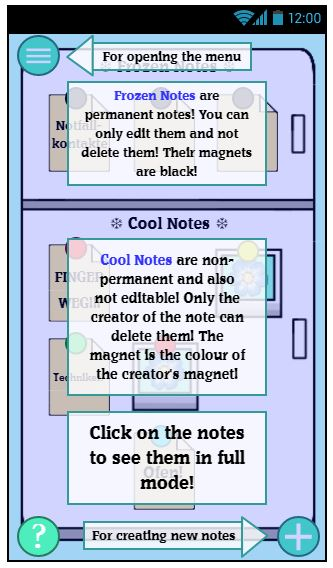
\includegraphics[width=0.7\textwidth]{fridget_tutorial.JPG}
    			\caption{Tutorial-Overlay}
    			\label{fig:figure1}
    		\end{minipage}
    		\hspace{0.5cm}
    		\begin{minipage}[t]{0.55\linewidth}
    			\flushleft
    			\vspace{9mm}
    			{[}S16{]} Tutorial-Overlay\\
    			\hfill
    			\\
    			Beschreibung: \\
    			Mehrere Textboxen mit Erklärungen der  
    			verschiedenen Elemente der
    			Pinnwand-View {[}S05{]}.
    			
    			\hfill 
    			\\Elemente:\\
    			\begin{itemize}
    				\renewcommand\labelitemi{--}
    				\item Textboxen mit Erklärungen
    				\item Hilfe-Button
    				
    			\end{itemize}
    			
    			
    			\hfill 
    			
    			Verwendung:\\
    			Das View dient als Tutorial für Leute, die Fridget
    			zum ersten Mal benutzen.\\ 
    			Durch das Tippen auf 
    			Hilfe-Button verschwindet das Overlay und man 
    			sieht wieder die normale Pinnwand-View {[}S05{]}.
    			
    		\end{minipage}
    	\end{figure}
    
    	\begin{figure}[h!]
    		\begin{minipage}[t]{0.45\linewidth}
    			\flushright
    			\centering
    			\vspace{9mm}
    			
\includegraphics[width=0.05\textheight]{menu_button.PNG}
    			\caption{{[}B01{]} Menü-Button}
    			\label{fig:figure1}
    			\hfill \\
    			
\includegraphics[width=0.05\textheight]{back_button.PNG}
    			\caption{{[}B02{]} Zurück-Button}
    			\label{fig:figure1}
    			\hfill \\
    			
\includegraphics[width=0.05\textheight]{minus_button.PNG}
    			\caption{{[}B03{]} Minus-Button}
    			\label{fig:figure1}
    			\end{minipage}
    			\hspace{0.5cm}
    			\begin{minipage}[t]{0.45\linewidth}
    			\flushright
    			\centering
    			\vspace{9mm}
    			
\includegraphics[width=0.05\textheight]{plus_button.PNG}
    			\caption{{[}B04{]} Plus-Button}
    			\label{fig:figure1}
    			\hfill \\
    			
\includegraphics[width=0.05\textheight]{edit_button.PNG}
    			\caption{{[}B05{]} Edit-Button}
    			\label{fig:figure1}
    			\hfill \\
    			
\includegraphics[width=0.05\textheight]{comment_button.PNG}
    			\caption{{[}B06{]} Kommentar-Button}
    			\label{fig:figure1}	
    				
    			\end{minipage}
    		\end{figure}
    
    	\clearpage

    \chapter{Testfälle}
    
    	\section{Basistestfälle - TB}    
    	
	    \begin{table}[h!]
	    	\centering
	    	\label{my-label}
	    	\begin{tabular}{p{2cm}p{12cm}}
	    		
	    		\multicolumn{2}{c}{\textbf{1 - Erstellen einer WG-Pinnwand}} \\ \hline
	    		\centering{[}TB1010{]} & Mit Google-Account registrieren {[}FG1010{]}\\
	    		\centering{[}TB1020{]}& Neue WG-Pinnwand erstellen {[}FG1020{]}                                \\
	    		\centering{[}TB1030{]} & Der neuerstellten WG-Pinnwand einen Namen geben {[}FG1020{]} \\ 
	    		\centering{[}TB1040{]}& Zugangscode generieren {[}FG1030{]}\\ 
	    		\centering{[}TB1050{]}& Anmelden mit Zugangscode {[}FG1050{]}\\ 
	    		\centering{[}TB1060{]}& \textit{Frozen Notes} automatisch generieren und anzeigen {[}FG1060{]}\\ 
	    		\hline
	    	\end{tabular}
	    \end{table}
	    
	    \vspace{5mm}
	    
	    \begin{table}[h!]
	    	\centering
	    	\label{my-label}
	    	\begin{tabular}{p{2cm}p{12cm}}
	    		
	    		\multicolumn{2}{c}{\textbf{2 - Interaktion mit der Pinnwand}} \\ \hline
	    		\centering{[}TB2010{]} & \textit{Cool Note} erstellen und eine Überschrift geben {[}FG2010{]}{[}FG2030{]}\\
	    		\centering{[}TB2020{]} & \textit{Cool Note} erstellen und im Text-Feld schreiben {[}FG2010{]}\\
	    		\centering{[}TB2030{]} & Textinhalte unterstreichen, kursiv-schreiben oder fett-drucken {[}FG2020{]}\\
	    		\centering{[}TB2040{]} & Eine \textit{Frozen-} oder \textit{Cool Note} antippen {[}FG2040{]}\\ 
	    		\centering{[}TB2050{]} & Eine \textit{Cool Note} mit Textinhalt und Überschrift löschen {[}FG2050{]}\\ 
	    		\centering{[}TB2060{]} & \textit{Frozen Note} bearbeiten {[}FG2040{]}\\ 
				\centering{[}TB2070{]} & 15 Mitglieder hinzufügen {[}FG2070{]}\\ 

	    		\centering{[}TB2080{]} & Die Pinnwand aktualisieren durch Hinunterswipen {[}FG2080{]}\\ 
	    		\hline
	    	\end{tabular}
	    \end{table}
	    
	    \vspace{5mm}
	    
	    \begin{table}[h!]
	    	\centering
	    	\label{my-label}
	    	\begin{tabular}{p{2cm}p{12cm}}
	    		
	    		\multicolumn{2}{c}{\textbf{3 - App-Menü}} \\ \hline
	    		\centering{[}TB3010{]} & Die WG verlassen {[}FG3010{]}\\
	    		\centering{[}TB3020{]} & Auf die Mitgliederliste zugreifen {[}FG3020{]}{[}FG3030{]}\\
	    		\hline
	    	\end{tabular}
	    \end{table}
	    
	    \vspace{5mm}
	    
	    \begin{table}[h!]
	    	\centering
	    	\label{my-label}
	    	\begin{tabular}{p{2cm}p{12cm}}
	    		
	    		\multicolumn{2}{c}{\textbf{4 - Lesebestätigung}} \\ \hline
	    		\centering{[}TB4010{]} & Auf die \textit{Cool Note} zugreifen nachdem alle Mitglieder sie  gelesen haben {[}FG4010{]}\\
	    		\centering{[}TB4030{]}& ``I have seen this"-Checkbox markieren {[}FG4030{]}\\ 
	    		
	    		\hline
	    	\end{tabular}
	    \end{table}
	    
	    \vspace{5mm}
	    
	    \begin{table}[h!]
	    	\centering
	    	\label{my-label}
	    	\begin{tabular}{p{2cm}p{12cm}}
	    		
	    		\multicolumn{2}{c}{\textbf{5 - Push-Benachrichtigung}} \\ \hline
	    		\centering{[}TB5010{]} & Push-Benachrichtigung antippen {[}FG5020{]}\\
	    		
	    		
	    		\hline
	    	\end{tabular}
	    \end{table}
	    
	    \clearpage
	    
	    \section{Erweiterte Testfälle - TE}
	    
	    \begin{table}[h]
	    	\centering
	    	\label{my-label}
	    	\begin{tabular}{p{2cm}p{12cm}}
	    		
	    		\multicolumn{2}{c}{\textbf{1 - Taggen}} \\ \hline
	    		\centering{[}TE1010{]} & Mitglieder mit ``@”-Zeichen taggen {[}FO1010{]}{[}FO1020{]}{[}KW1020{]}\\
	    		\hline
	    	\end{tabular}
	    \end{table}
	    
	    \vspace{5mm}
	    
	    \begin{table}[h!]
	    	\centering
	    	\label{my-label}
	    	\begin{tabular}{p{2cm}p{12cm}}
	    		
	    		\multicolumn{2}{c}{\textbf{2 - Interaktion mit der Pinnwand}} \\ \hline
	    		\centering{[}TE2010{]} & Zettelfarbe festlegen {[}FO2010{]}\\
	    		\centering{[}TE2020{]}& Eine \textit{Cool Note}  mit Bildinhalt und Beschreibung erstellen {[}FO2020{]}                             \\
	    		\centering{[}TE2030{]}& Eine \textit{Cool Note} mit Bildinhalt und Beschreibung löschen {[}FO2030{]}\\ 
	    		\centering{[}TE2040{]}& Eine \textit{Cool Note} kommentieren {[}F02040{]}  \\ 
	    		\centering{[}TE2050{]}& Eine \textit{Cool Note} archivieren {[}F02050{]}\\ 
	    		\centering{[}TE2060{]}& Durch die Kommentare scrollen {[}F02060{]}\\ 
	    		\hline
	    	\end{tabular}
	    \end{table}
	    
	    \vspace{5mm}
	    
	    \begin{table}[h!]
	    	\centering
	    	\label{my-label}
	    	\begin{tabular}{p{2cm}p{12cm}}
	    		
	    		\multicolumn{2}{c}{\textbf{3 - App Einstellungen / App-Menü}} \\ \hline
	    		\centering{[}TE3010{]} & Die Sprache der App umstellen {[}FO3010{]}\\
	    		\centering{[}TE3020{]} & Das \textit{Cool-Note}-Archiv aufrufen und durchscrollen {[}FO3020{]}\\
	    		\hline
	    	\end{tabular}
	    \end{table}
	    
	    \vspace{5mm}
	    
	    \begin{table}[h!]
	    	\centering
	    	\label{my-label}
	    	\begin{tabular}{p{2cm}p{12cm}}
	    		
	    		\multicolumn{2}{c}{\textbf{4 - Hilfe-Button / ``Tutorial"}} \\ \hline
	    		\centering{[}TE4010{]} & Das Tutorial-Overlay ansehen {[}FO4010{]}\\    				
	    		\hline
	    	\end{tabular}
	    \end{table}
	    
	   
	    
	    \clearpage
	    
	  	\section{Testszenarien}
	  	
	  	\begin{table}[h!]
	  		\centering
	  		\label{my-label}
	  		\begin{tabular}{p{2cm}p{12cm}}
	  			
	  			\multicolumn{2}{c}{\textbf{{[}TS01{]} - Erste Benutzung der App}} \\ \hline
	  			\multicolumn{2}{p\linewidth}{Die Bewohner einer WG entscheidet sich die App zu benutzen. Einer von ihnen registriert ihre WG und gibt den Zugangscode den anderen weiter. Sie registrieren sich alle mit ihrem Google-Account und gelangen zu ihrer WG-Pinnwand, wo sie zunächst sich das Tutorial anschauen.} 
	  			\vspace{7mm}\\
	  			\centering{[}TB1010{]} & Mit Google-Account registrieren\\
	  			\centering{[}TB1020{]}& Neue WG-Pinnwand erstellen    \\
	  			\centering{[}TB1030{]} & Der neuerstellten WG-Pinnwand einen Namen geben \\ 
	  			\centering{[}TB1040{]}& Zugangscode generieren \\ 
	  			\centering{[}TB1050{]}& Anmelden mit Zugangscode\\ 
	  			\centering{[}TB2070{]}& 15 Mitglieder hinzufügen\\ 
	  			\centering{[}TE4010{]} & Das Tutorial-Overlay ansehen \\
	  			\hline
	  		\end{tabular}
	  	\end{table}
  		
  		\vspace{1cm}
  		
  		\begin{table}[h!]
  			\centering
  			\label{my-label}
  			\begin{tabular}{p{2cm}p{12cm}}
  				
  				\multicolumn{2}{c}{\textbf{{[}TS02{]} - Erstellung einer \textit{Cool Note}}} \\ \hline
  				\multicolumn{2}{p{\linewidth}}{Ein Mitglied erstellt eine \textit{Cool Note} mit einer Frage, welches er direkt an einem seiner Mitbewohner richten möchte. Er taggt diesen. Kurz darauf merkt er, dass er die Frage doch an alle richten möchte. Er löscht die \textit{Cool Note}, archiviert diesen und erstellt eine neue \textit{Cool Note}. Da für ihm die Notiz sehr dringend ist, achtet er darauf, wer die Note schon alles gelesen hat und sie kommentiert hat. Die anderen Mitglieder erhalten eine Push-Benachrichtigung und öffnen die \textit{Cool Note} sofort.} 
  				\vspace{7mm}\\
  				
  				\centering{[}TB2010{]} & \textit{Cool Note} erstellen und eine Überschrift geben \\
  				\centering{[}TB2020{]} & \textit{Cool Note} erstellen und im Text-Feld schreiben \\
  				\centering{[}TB2030{]} & Textinhalte unterstreichen, kursiv-schreiben oder fett-drucken\\
  				\centering{[}TB2040{]} & Eine \textit{Frozen-} oder \textit{Cool Note} antippen \\ 
  				\centering{[}TB2050{]} & Eine \textit{Cool Note} mit Textinhalt und Überschrift löschen \\ 
  				\centering{[}TB4010{]} & Auf die \textit{Cool Note} zugreifen nachdem alle Mitglieder sie  gelesen haben \\
  				\centering{[}TB5010{]} & Push-Benachrichtigung antippen \\
  				\centering{[}TE1010{]} & Mitglieder mit ``@”-Zeichen taggen\\
  				\centering{[}TE2010{]} & Zettelfarbe festlegen \\
  				\centering{[}TE2040{]}& Eine \textit{Cool Note} kommentieren   \\ 
  				\centering{[}TE2050{]}& Eine \textit{Cool Note} archivieren\\ 
  				\centering{[}TE2060{]}& Durch die Kommentare scrollen\\ 
  				
  				\hline
  			\end{tabular}
  		\end{table}
  	
	  	\begin{table}[h!]
	  		\centering
	  		\label{my-label}
	  		\begin{tabular}{p{2cm}p{12cm}}
	  			
	  			\multicolumn{2}{c}{\textbf{{[}TS03{]} - Bearbeitung einer \textit{Frozen Note}}} \\ \hline
	  			\multicolumn{2}{p\linewidth}{Ein WG-Mitglied tippt auf eine leere \textit{Frozen Note} und sieht die Großansicht. Es möchte sie bearbeiten und tippt auf den Edit-Button. Dadurch öffnet sich die Edit-Ansicht. Es kann nun der \textit{Frozen Note} eine Überschrift geben und den Inhalt schreiben. Durch das Antippen des ``Post it!”-Buttons, werden die Änderungen gespeichert und das Mitglied sieht seine editierte \textit{Frozen Note} in der Großansicht.}
	  			\vspace{7mm} \\
	  			\centering{[}TB2040{]} & Eine \textit{Frozen Note} antippen\\
	  			\centering{[}TB2060{]}& \textit{Frozen Note} bearbeiten    \\
	  			\hline
	  		\end{tabular}
	  	\end{table}
  	
  		\begin{table}[h!]
  			\centering
  			\label{my-label}
  			\begin{tabular}{p{2cm}p{12cm}}
  				
  				\multicolumn{2}{c}{\textbf{{[}TS04{]} - Verlassen der WG}} \\ \hline
  				\multicolumn{2}{p\linewidth}{WG-Mitglied A möchte die WG verlassen und tippt auf den Menüpunkt ``Leave flatshare”. WG-Mitglied B aktualisiert die Pinnwand manuell und sieht nun, dass alle \textit{Cool Notes} des Verlassenden gelöscht wurden. Danach öffnet WG-Mitglied B das Menü und sieht unter dem Menüpunkt ``Members”, dass die Mitgliederliste aktualisiert wurde und der Name von Mitglied A sowie der zugehörige Magnet entfernt wurden.}
  				\vspace{7mm} \\
  				\centering{[}TB3010{]} & Die WG verlassen\\
  				\centering{[}TB3020{]}& Auf die Mitgliederliste zugreifen  \\
  				\hline
  			\end{tabular}
  		\end{table}
	  	
    
    \chapter{Entwicklungsumgebung}
    
    \begin{table}[h!]
    	\centering
    	\label{my-label}
    	\begin{tabular}{p{5.5cm}p{8.5cm}}
    		
    		\multicolumn{2}{c}{\textbf{1 - Software}} \\ \hline
    		Entwicklungsumgebung & Android Studio 3.1.2\\
    		Graphische Oberfläche& Evolus Pencil                               \\
    		Versionierung & Git \\
    		Dokumentation & TeXstudio \newline Microsoft Powerpoint \newline Microsoft Word \\
    		\hline
    	\end{tabular}
    \end{table}
    
    \vspace{5mm}
    
    \begin{table}[h!]
    	\centering
    	\label{my-label}
    	\begin{tabular}{p{5.5cm}p{8.5cm}}
    		
    		\multicolumn{2}{c}{\textbf{2 - Hardware}} \\ \hline
    		Lenovo G570 & Intel Core i5 2410M / 2.3 GHz \newline 8GB DDR3 SDRAM \newline 64-bit Ubuntu 16.04\\
    		Toshiba Satellite \newline L50-B-2H8 & Intel Core i5 5200U / 2.2 GHz \newline 8GB DDR3L RAM \newline 64-bit Windows 10                              \\
    		MacBook Pro & Intel Core i5 5257U / 2.7 GHz \newline 8GB DDR3 SDRAM \newline macOS High Sierra 10.13.3\\ 
    		Toshiba Satellite \newline L50-C-1K4 & Intel Core i7 5500U / 2.40 GHz \newline 8GB DDR3L RAM \newline 64-bit Windows 10\\ 
    		Samsung G. Book & Intel Core i5 7200U / 2.5 GHz \newline 8GB LPDDR3-1867 RAM \newline 64-bit Windows 10 Pro \\
    		\hline
    	\end{tabular}
    \end{table}

	\chapter{Glossar}
	
    \glsaddall
    \printglossaries

    \listoffigures

\end{document}